\documentclass[11pt, a4paper]{article}
\usepackage{pdfpages}
\usepackage{parallel}
\usepackage[T2A]{fontenc}
\usepackage{ucs}
\usepackage[utf8x]{inputenc}
\usepackage[polish,english,russian]{babel}
\usepackage{hyperref}
\usepackage{rotating}
\usepackage[inner=2cm,top=1.8cm,outer=2cm,bottom=2.3cm,nohead]{geometry}
\usepackage{listings}
\usepackage{graphicx}
\usepackage{wrapfig}
\usepackage{longtable}
\usepackage{indentfirst}
\usepackage{array}
\usepackage{tikzsymbols}
\usepackage{soul}
\usepackage[ruled,vlined]{algorithm2e}
%\counterwithout{figure}{section} 

\usepackage{url}
\makeatletter
\g@addto@macro{\UrlBreaks}{\UrlOrds}
\makeatother

\newcolumntype{P}[1]{>{\raggedright\arraybackslash}p{#1}}
\frenchspacing
\usepackage{fixltx2e} %text sub- and superscripts
\usepackage{icomma} % коскі ў матэматычным рэжыме
\PreloadUnicodePage{4}

\newcommand{\longpage}{\enlargethispage{\baselineskip}}
\newcommand{\shortpage}{\enlargethispage{-\baselineskip}}

\def\switchlang#1{\expandafter\csname switchlang#1\endcsname}
\def\switchlangbe{
\let\saverefname=\refname%
\def\refname{Літаратура}%
\def\figurename{Іл.}%
}
\def\switchlangen{
\let\saverefname=\refname%
\def\refname{References}%
\def\figurename{Fig.}%
}
\def\switchlangru{
\let\saverefname=\refname%
\let\savefigurename=\figurename%
\def\refname{Литература}%
\def\figurename{Рис.}%
}

\hyphenation{admi-ni-stra-tive}
\hyphenation{ex-pe-ri-ence}
\hyphenation{fle-xi-bi-li-ty}
\hyphenation{Py-thon}
\hyphenation{ma-the-ma-ti-cal}
\hyphenation{re-ported}
\hyphenation{imp-le-menta-tions}
\hyphenation{pro-vides}
\hyphenation{en-gi-neering}
\hyphenation{com-pa-ti-bi-li-ty}
\hyphenation{im-pos-sible}
\hyphenation{desk-top}
\hyphenation{elec-tro-nic}
\hyphenation{com-pa-ny}
\hyphenation{de-ve-lop-ment}
\hyphenation{de-ve-loping}
\hyphenation{de-ve-lop}
\hyphenation{da-ta-ba-se}
\hyphenation{plat-forms}
\hyphenation{or-ga-ni-za-tion}
\hyphenation{pro-gramming}
\hyphenation{in-stru-ments}
\hyphenation{Li-nux}
\hyphenation{sour-ce}
\hyphenation{en-vi-ron-ment}
\hyphenation{Te-le-pathy}
\hyphenation{Li-nux-ov-ka}
\hyphenation{Open-BSD}
\hyphenation{Free-BSD}
\hyphenation{men-ti-on-ed}
\hyphenation{app-li-ca-tion}

\def\progref!#1!{\texttt{#1}}
\renewcommand{\arraystretch}{2} %Іначай формулы ў матрыцы зліпаюцца з лініямі
\usepackage{array}

\def\interview #1 (#2), #3, #4, #5\par{

\section[#1, #3, #4]{#1 -- #3, #4}
\def\qname{LVEE}
\def\aname{#1}
\def\q ##1\par{{\noindent \bf \qname: ##1 }\par}
\def\a{{\noindent \bf \aname: } \def\qname{L}\def\aname{#2}}
}

\def\interview* #1 (#2), #3, #4, #5\par{

\section*{#1\\{\small\rm #3, #4. #5}}
\ifx\ParallelWhichBox\undefined%
    \addcontentsline{toc}{section}{#1, #3, #4}%
\else%
\ifnum\ParallelWhichBox=0%
    \addcontentsline{toc}{section}{#1, #3, #4}%
\fi\fi%

\def\qname{LVEE}
\def\aname{#1}
\def\q ##1\par{{\noindent \bf \qname: ##1 }\par}
\def\a{{\noindent \bf \aname: } \def\qname{L}\def\aname{#2}}
}

\newcommand{\interviewfooter}[1]{
\vskip 1em
\noindent \textit{#1}
}


\begin{document}

\title{1997 "--- Fellowes Sphere Trackball}
\date{}
\maketitle

Fellowes Sphere Trackball, показанный на рис. \ref{fig:FellowesTrackballPic} — типичный представитель данного типа указательных устройств ввода информации для компьютера, наиболее характерных для первой половины 90-х годов (хотя и выпущен компанией Fellowes Computerware в 1997).

\begin{figure}[h]
    \centering
    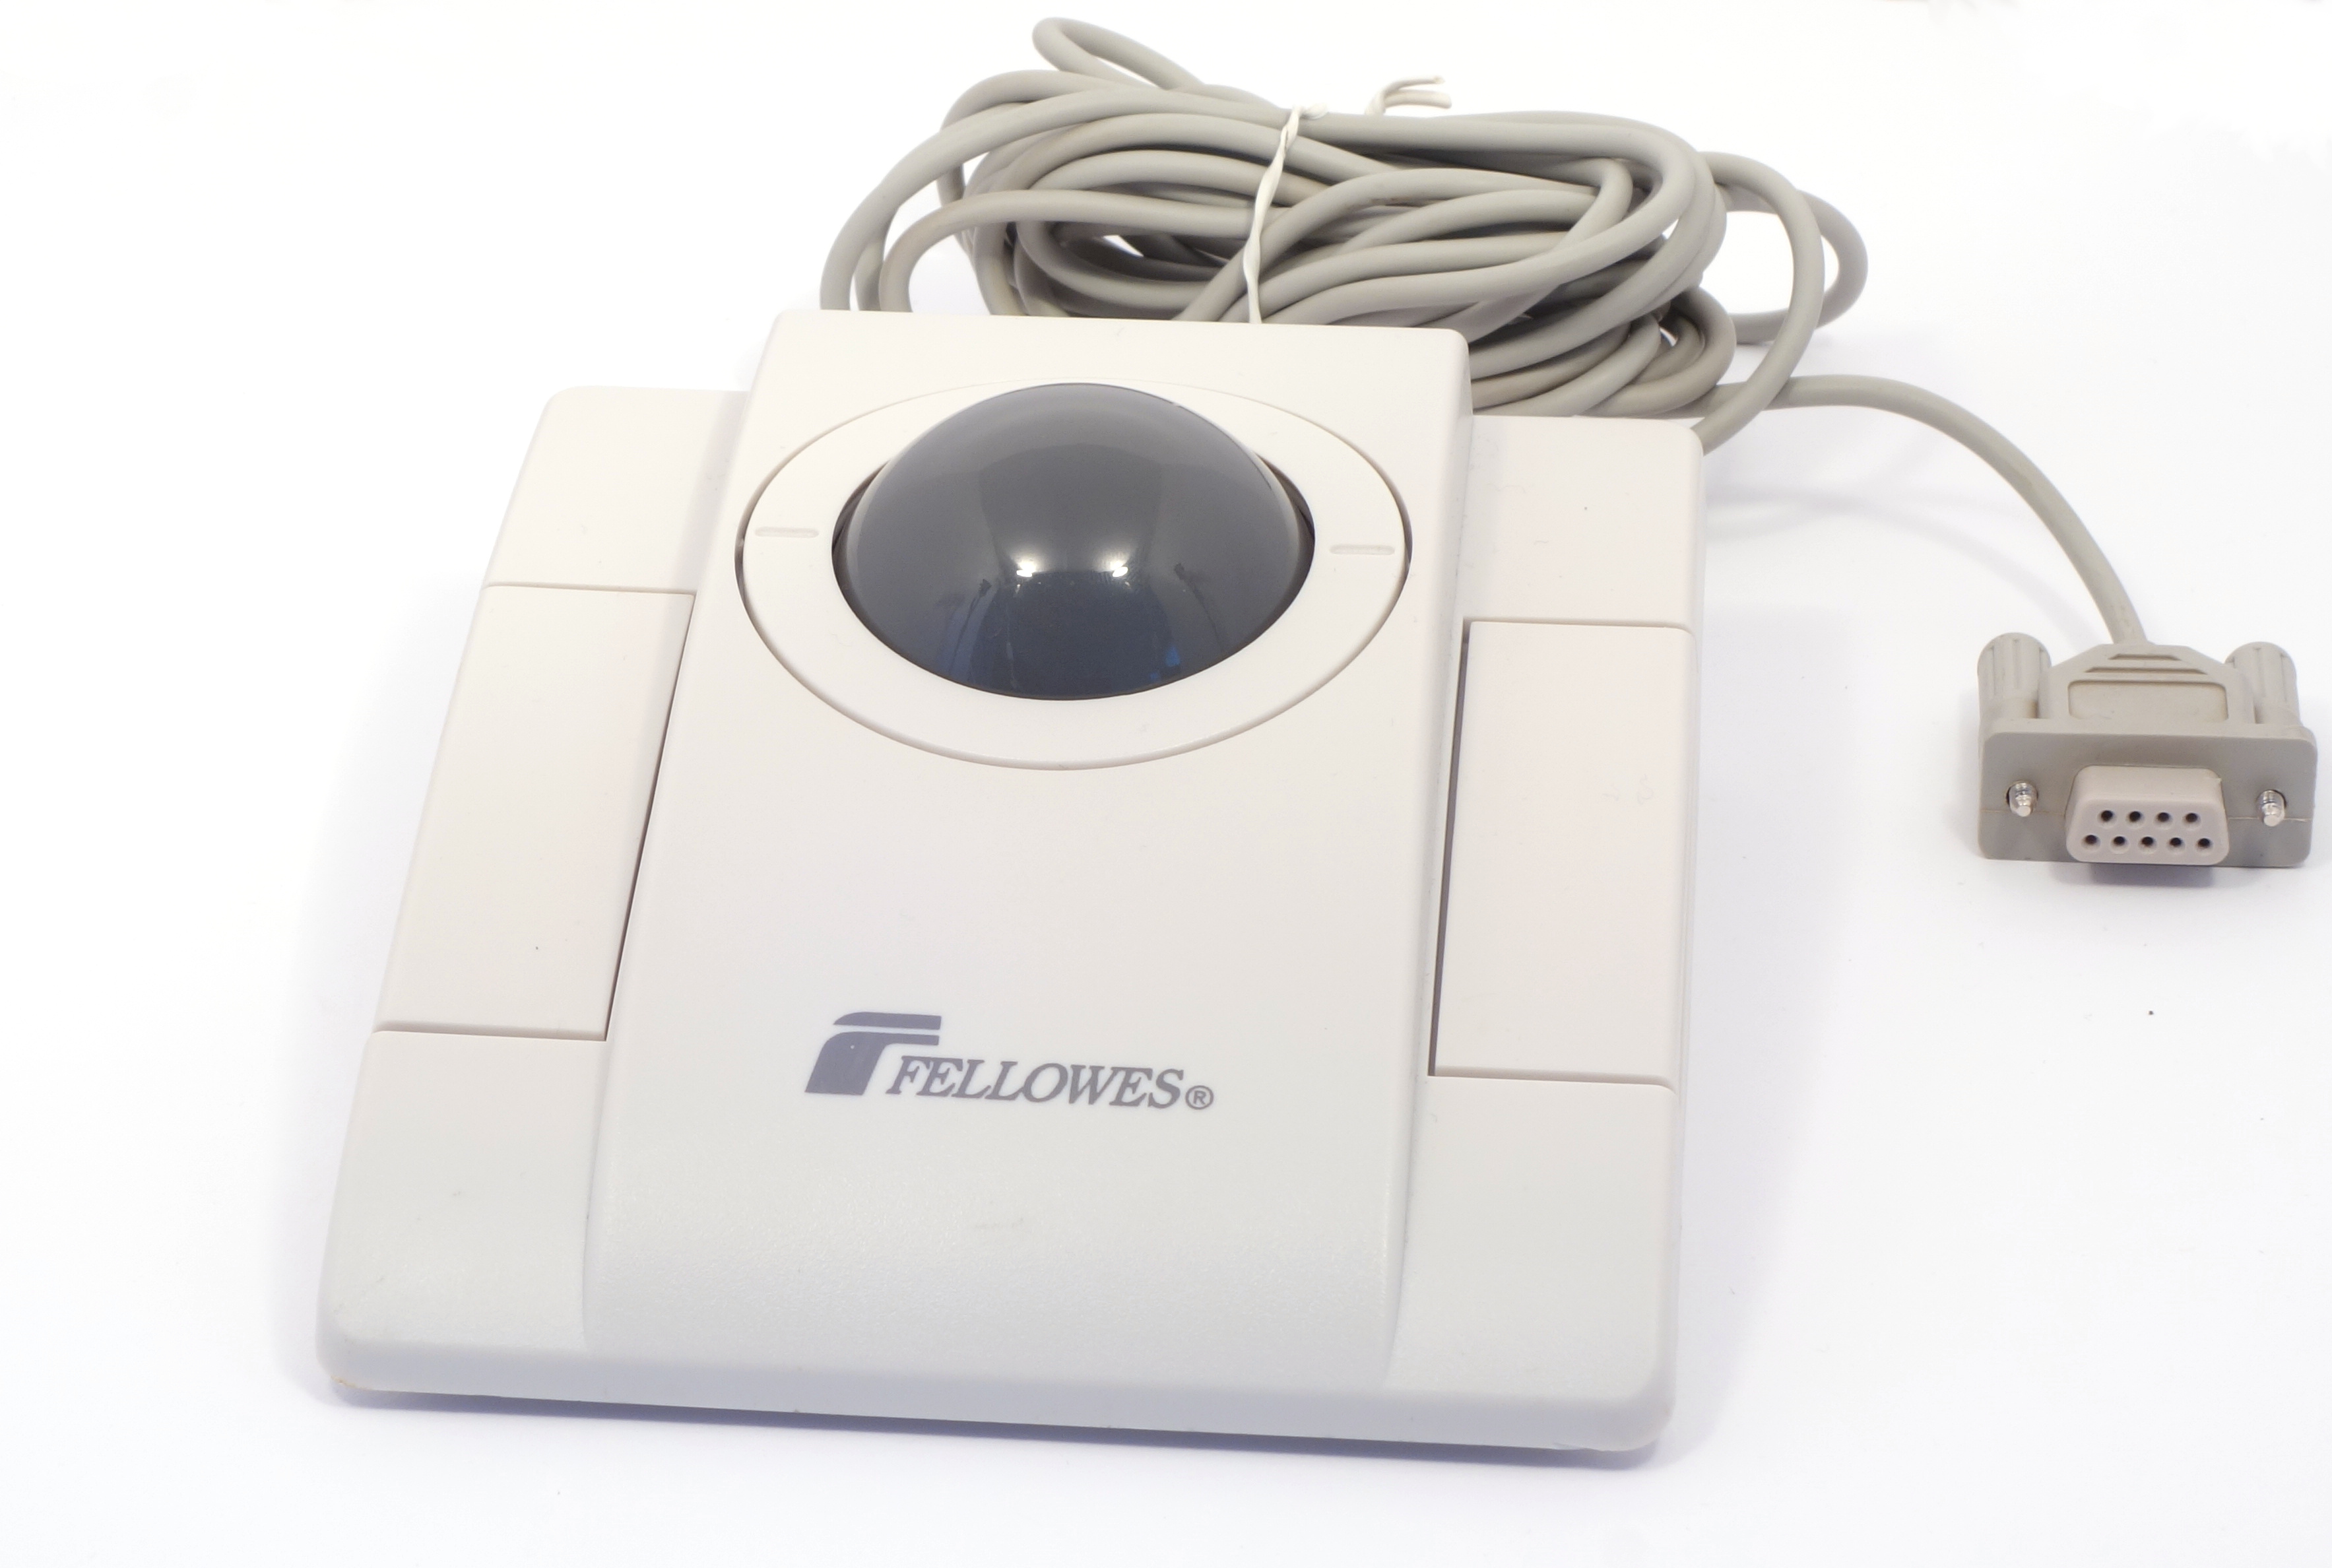
\includegraphics[scale=0.5]{1997_fellowes_trackball/pic_30.jpg}
    \caption{Fellowes Trackball}
    \label{fig:FellowesTrackballPic}
\end{figure}

Этот трекбол имеет симметричный дизайн, подходящий как для правшей, так и для левшей (рис. \ref{fig:FellowesTrackballTopBottom}). 

\begin{figure}[h]
    \centering
    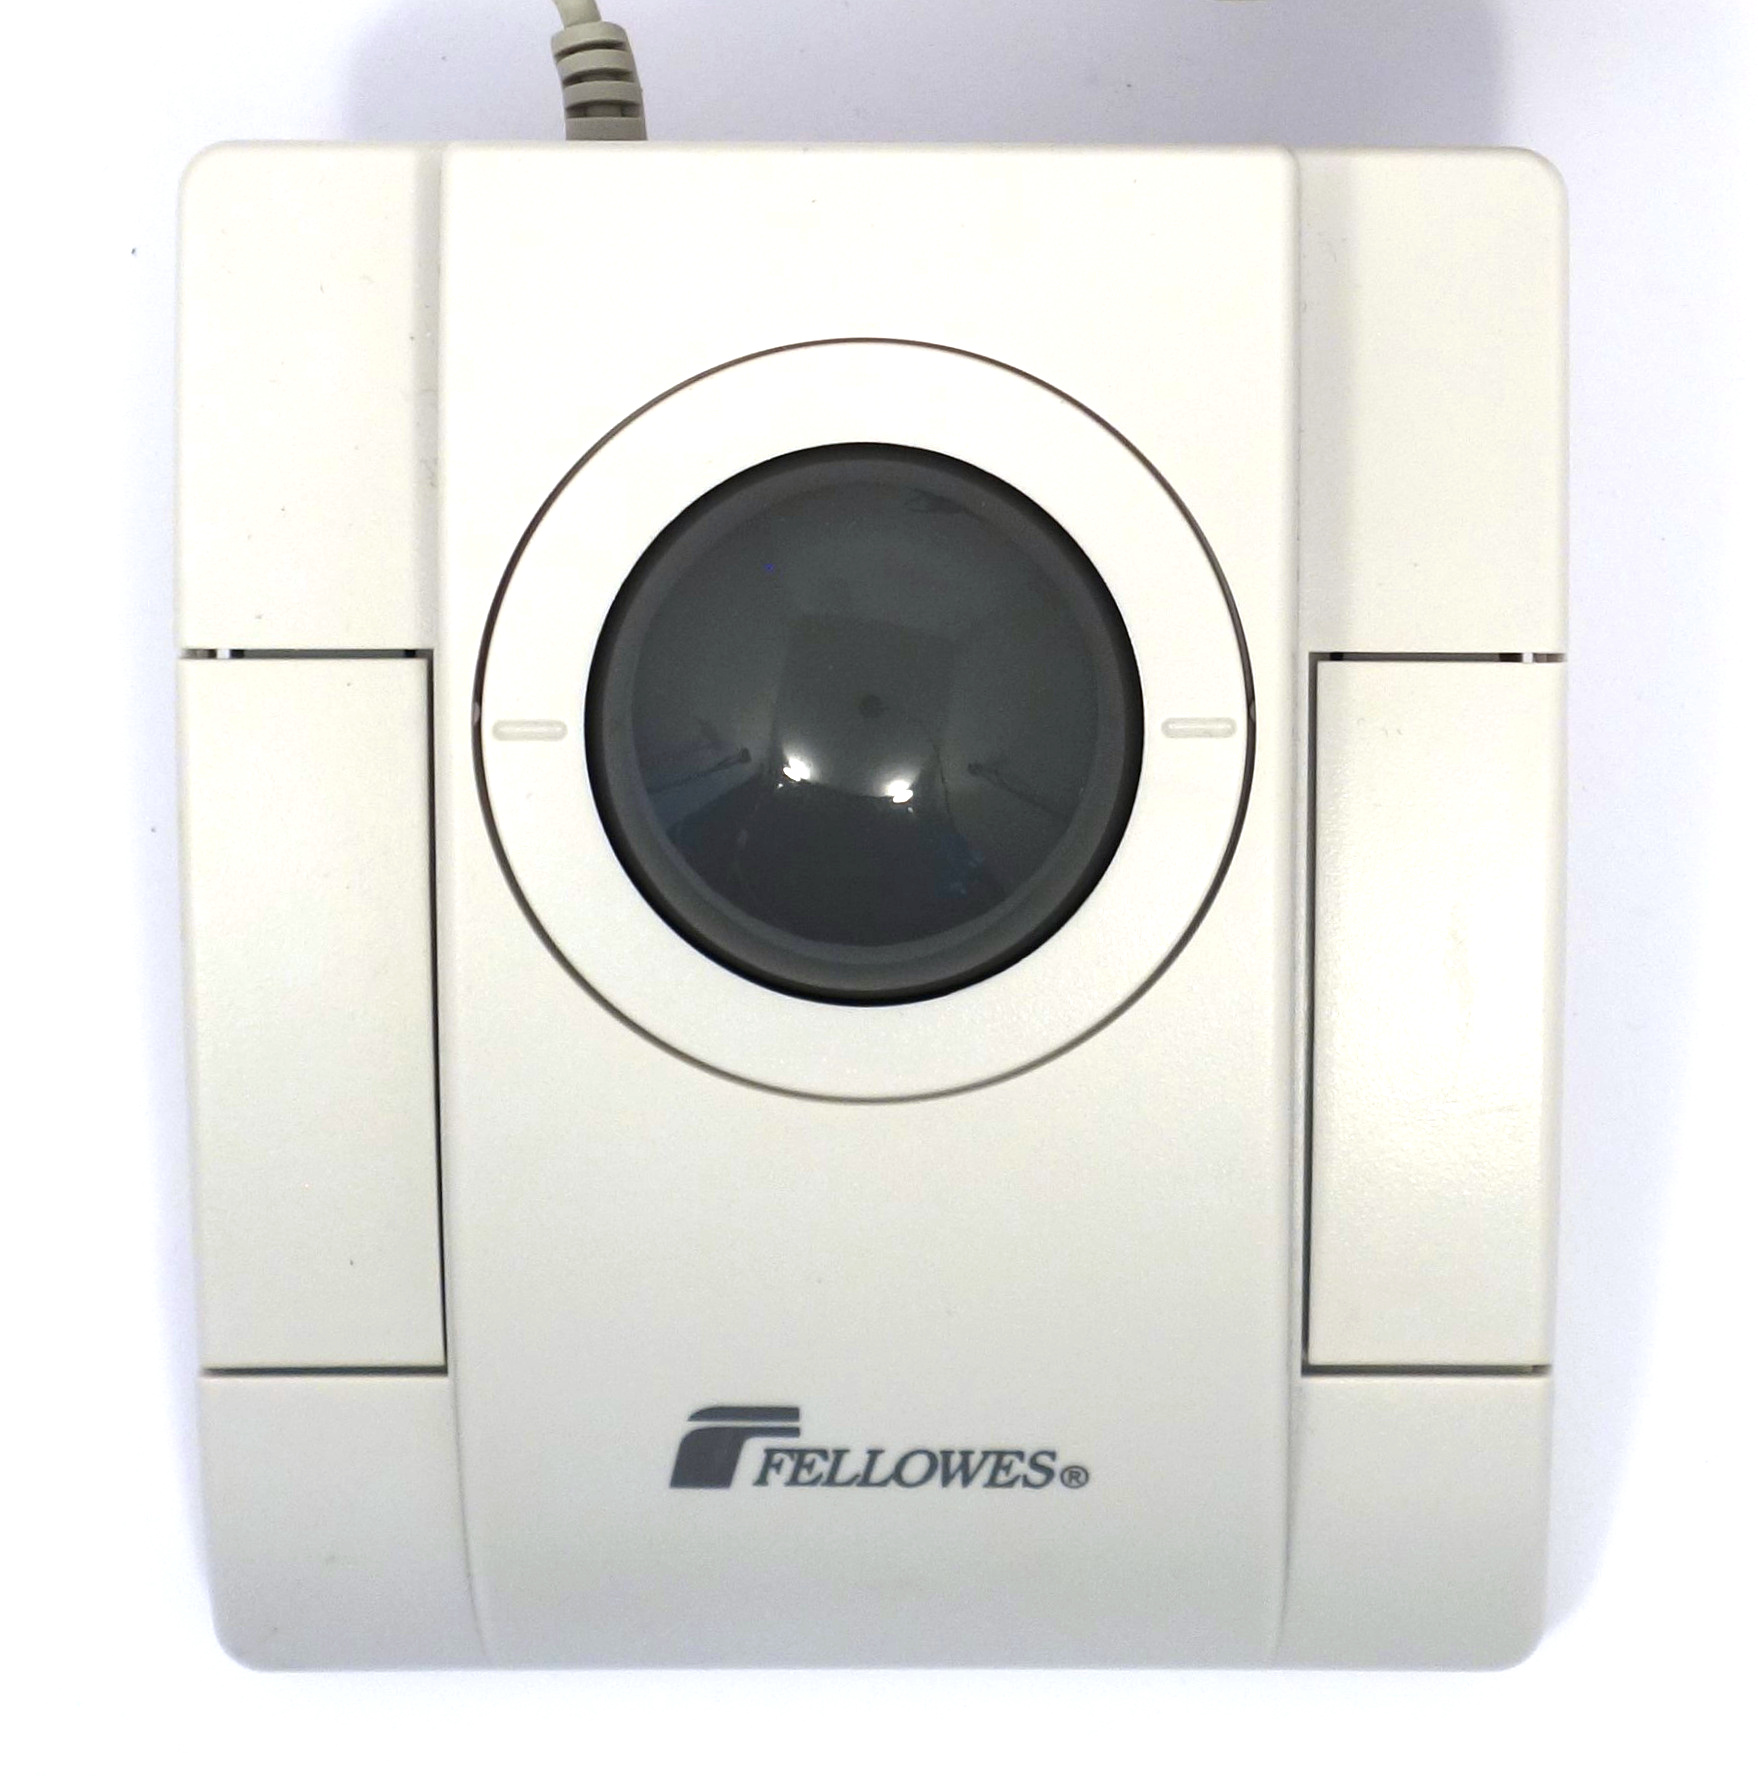
\includegraphics[scale=0.45]{1997_fellowes_trackball/top_60.jpg}
    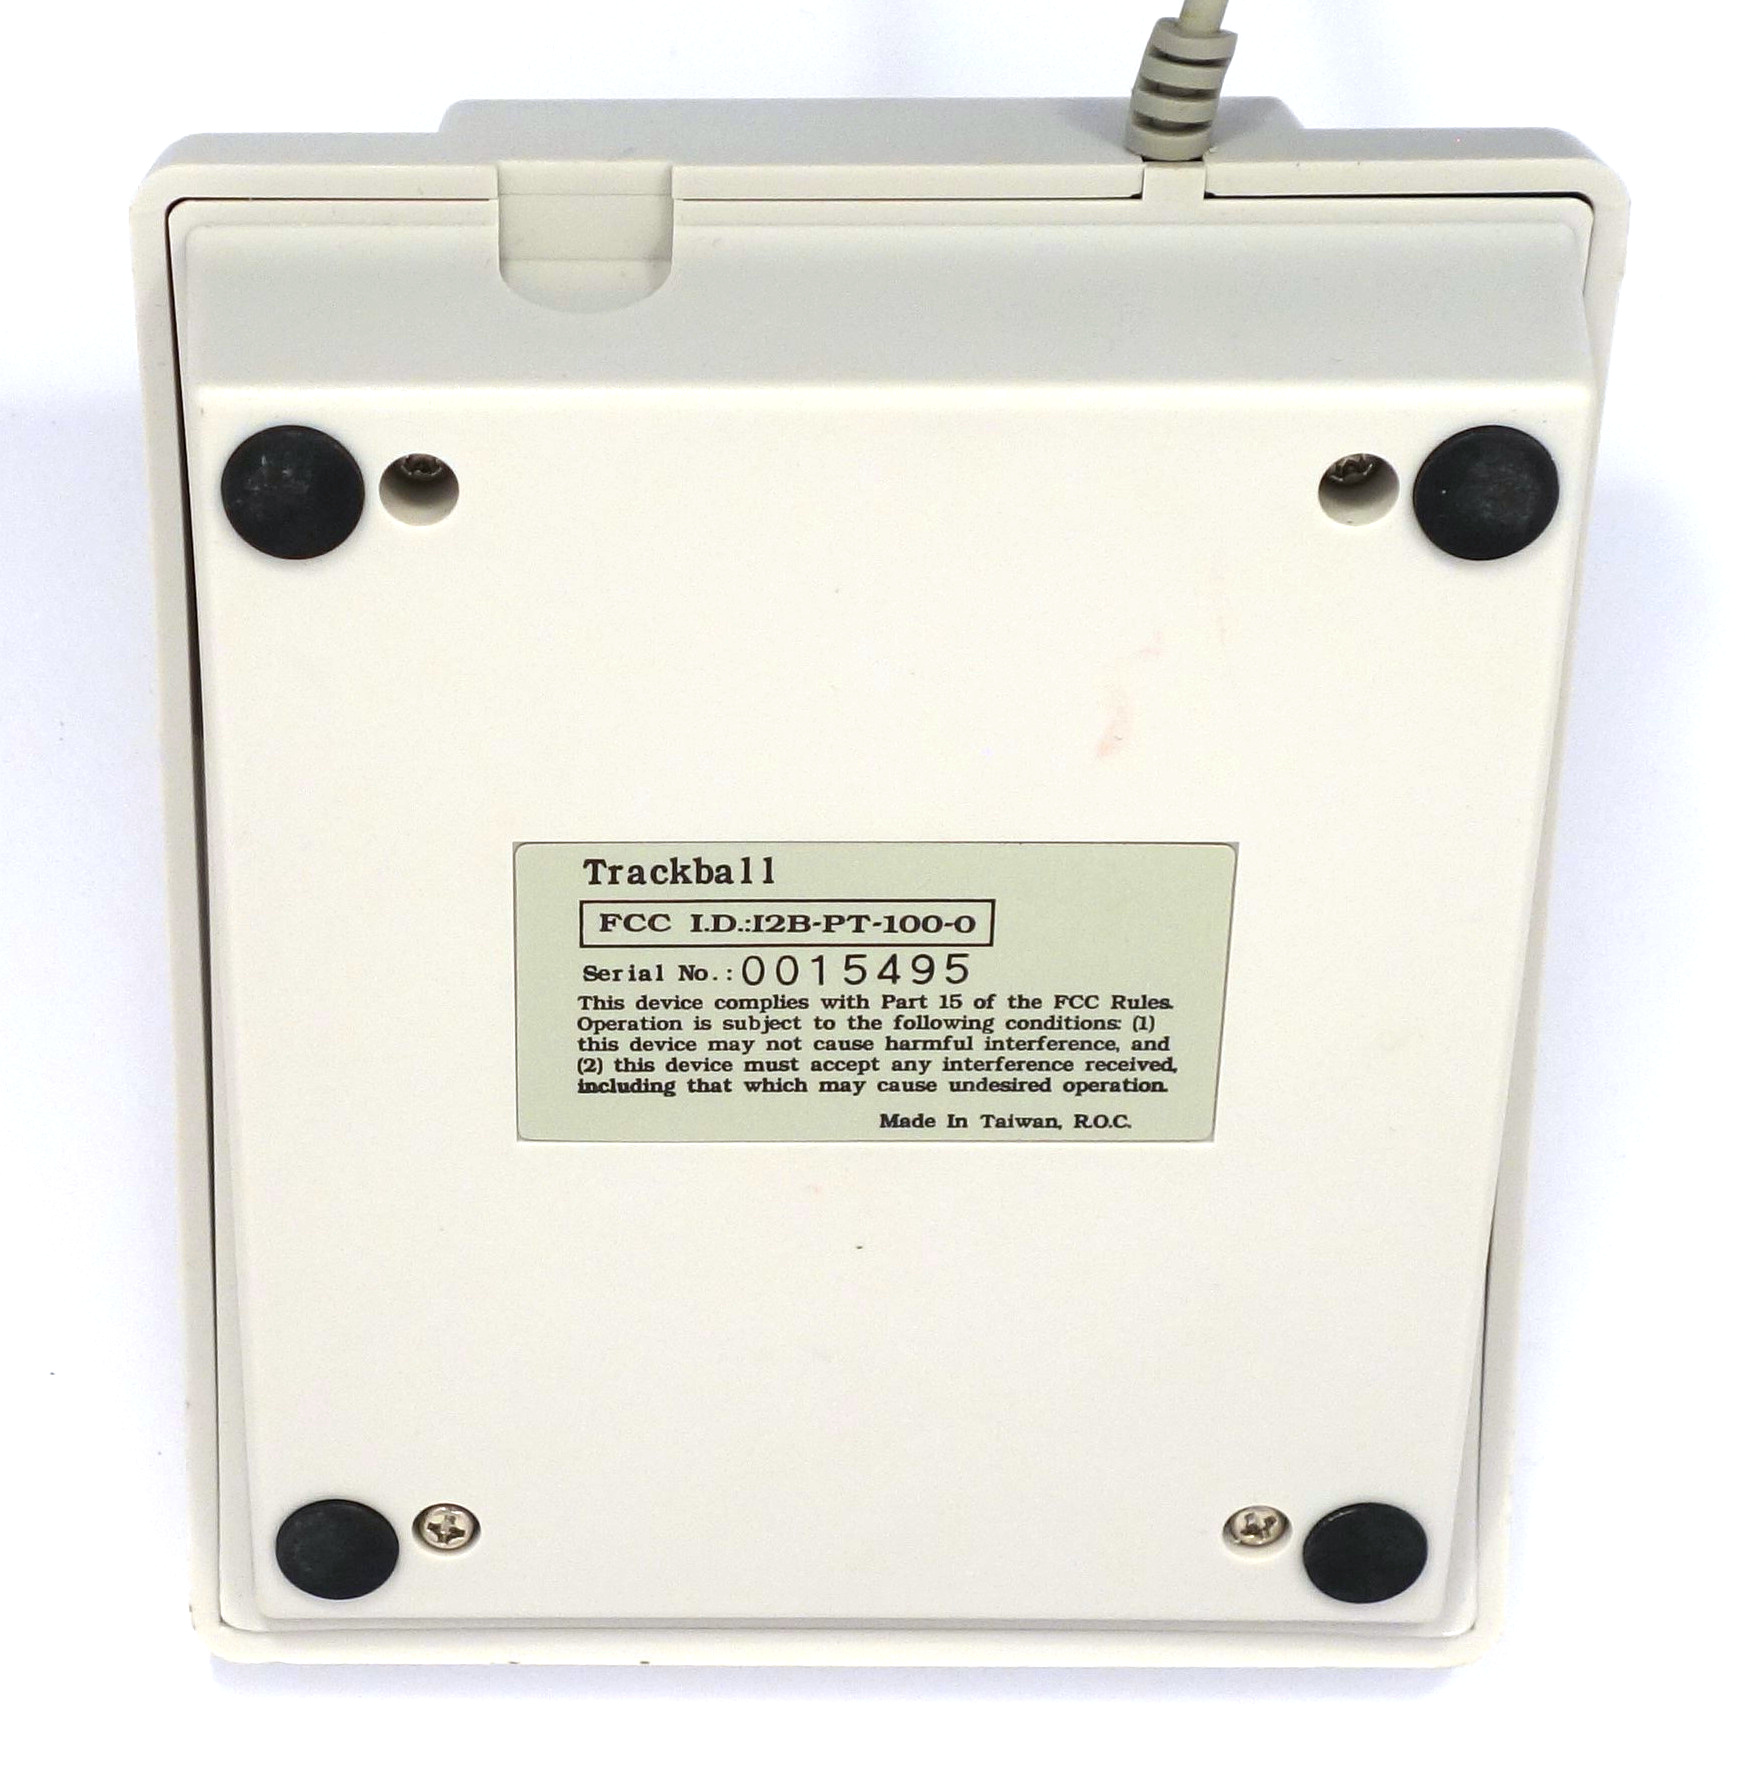
\includegraphics[scale=0.45]{1997_fellowes_trackball/bottom_60.jpg}
    \caption{Fellowes Trackball, вид сверху и снизу}
    \label{fig:FellowesTrackballTopBottom}
\end{figure}

Трекбол является достаточно крупным (рис. \ref{fig:FellowesTrackballSize}); в описании, приведенном в каталоге производителя, в качестве отличительных особенностей устройства упоминается прецизионное управление, достигаемое за счёт шара большого диаметра, а также легкое извлечение шара для чистки \cite{advertising}.

\begin{figure}[h]
    \centering
    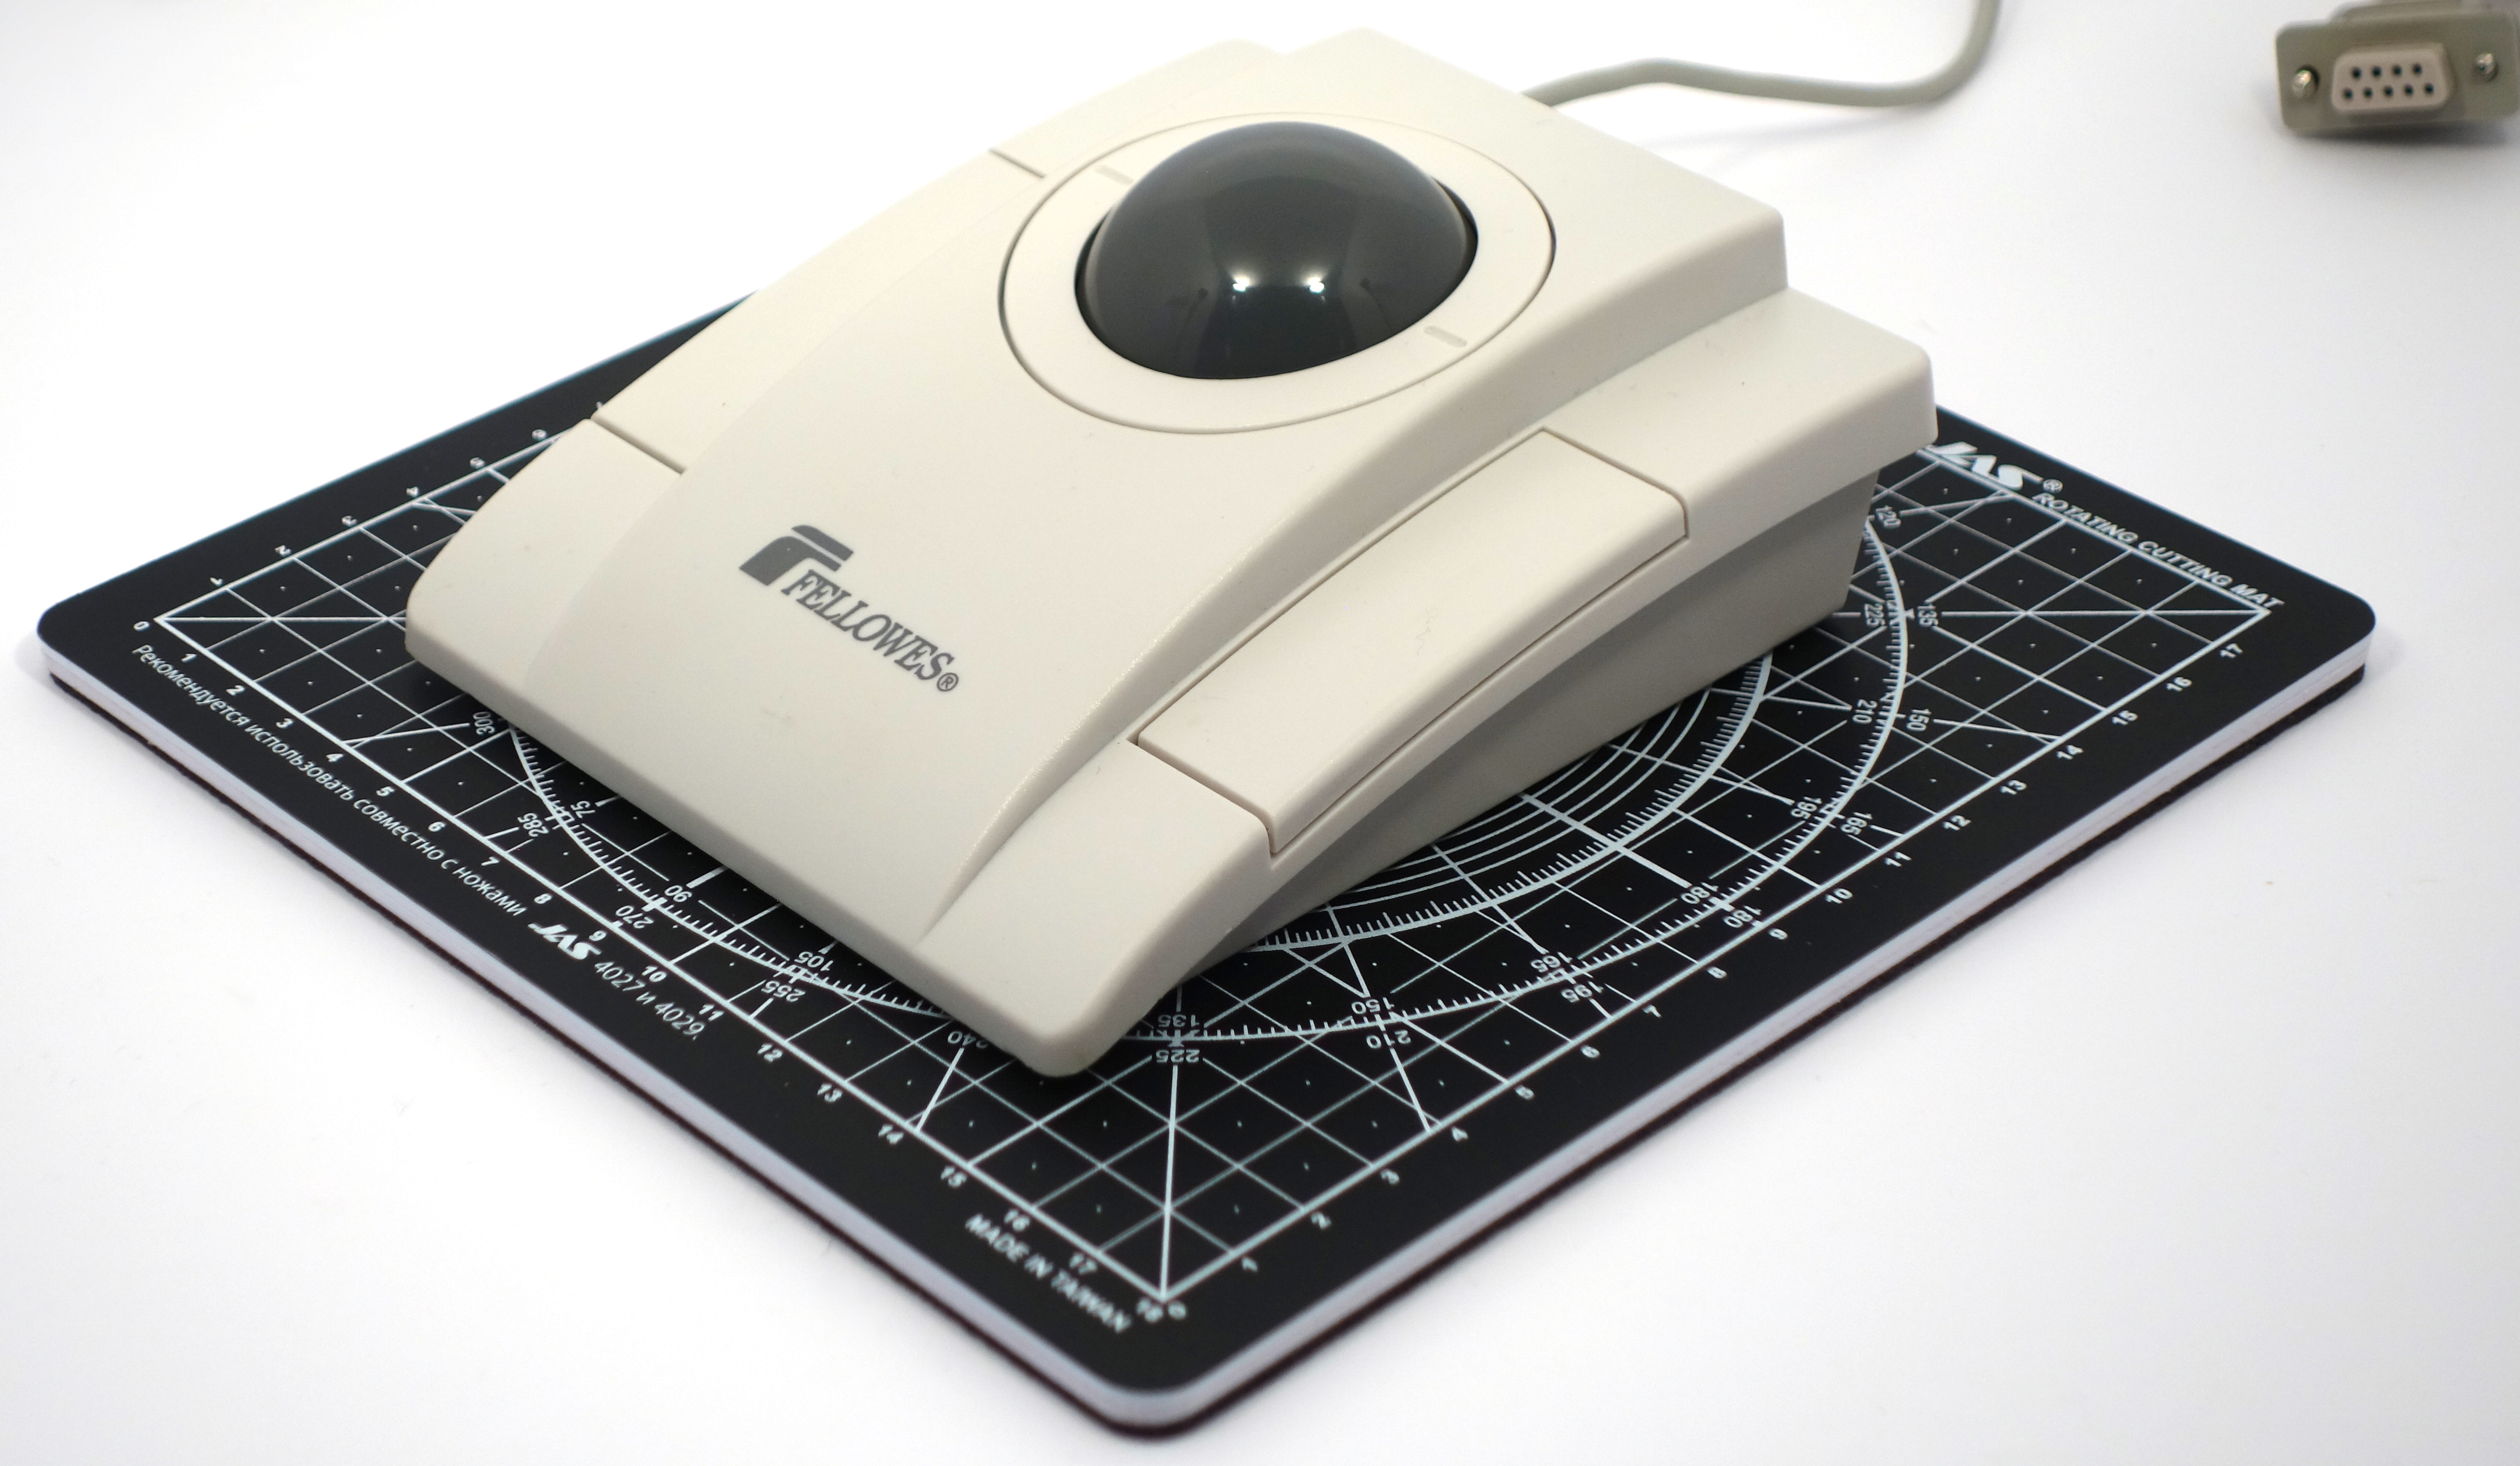
\includegraphics[scale=0.3]{1997_fellowes_trackball/size_30.jpg}
    \caption{Fellowes Trackball на размерном коврике с шагом сетки 1~см}
    \label{fig:FellowesTrackballSize}
\end{figure}

При работе с трекболом для операций перемещения курсора используется только кисть руки и движения пальцев. Поэтому от пользователя не требуется движений плеча и предплечья, тогда как те же операции с мышью требуют задействования практически всей руки. Поэтому трекбол часто рекомендуется пользователям, испытывающим временные или постоянные проблемы, связанные сплечевым поясом или запястьем.

\begin{figure}[h]
    \centering
    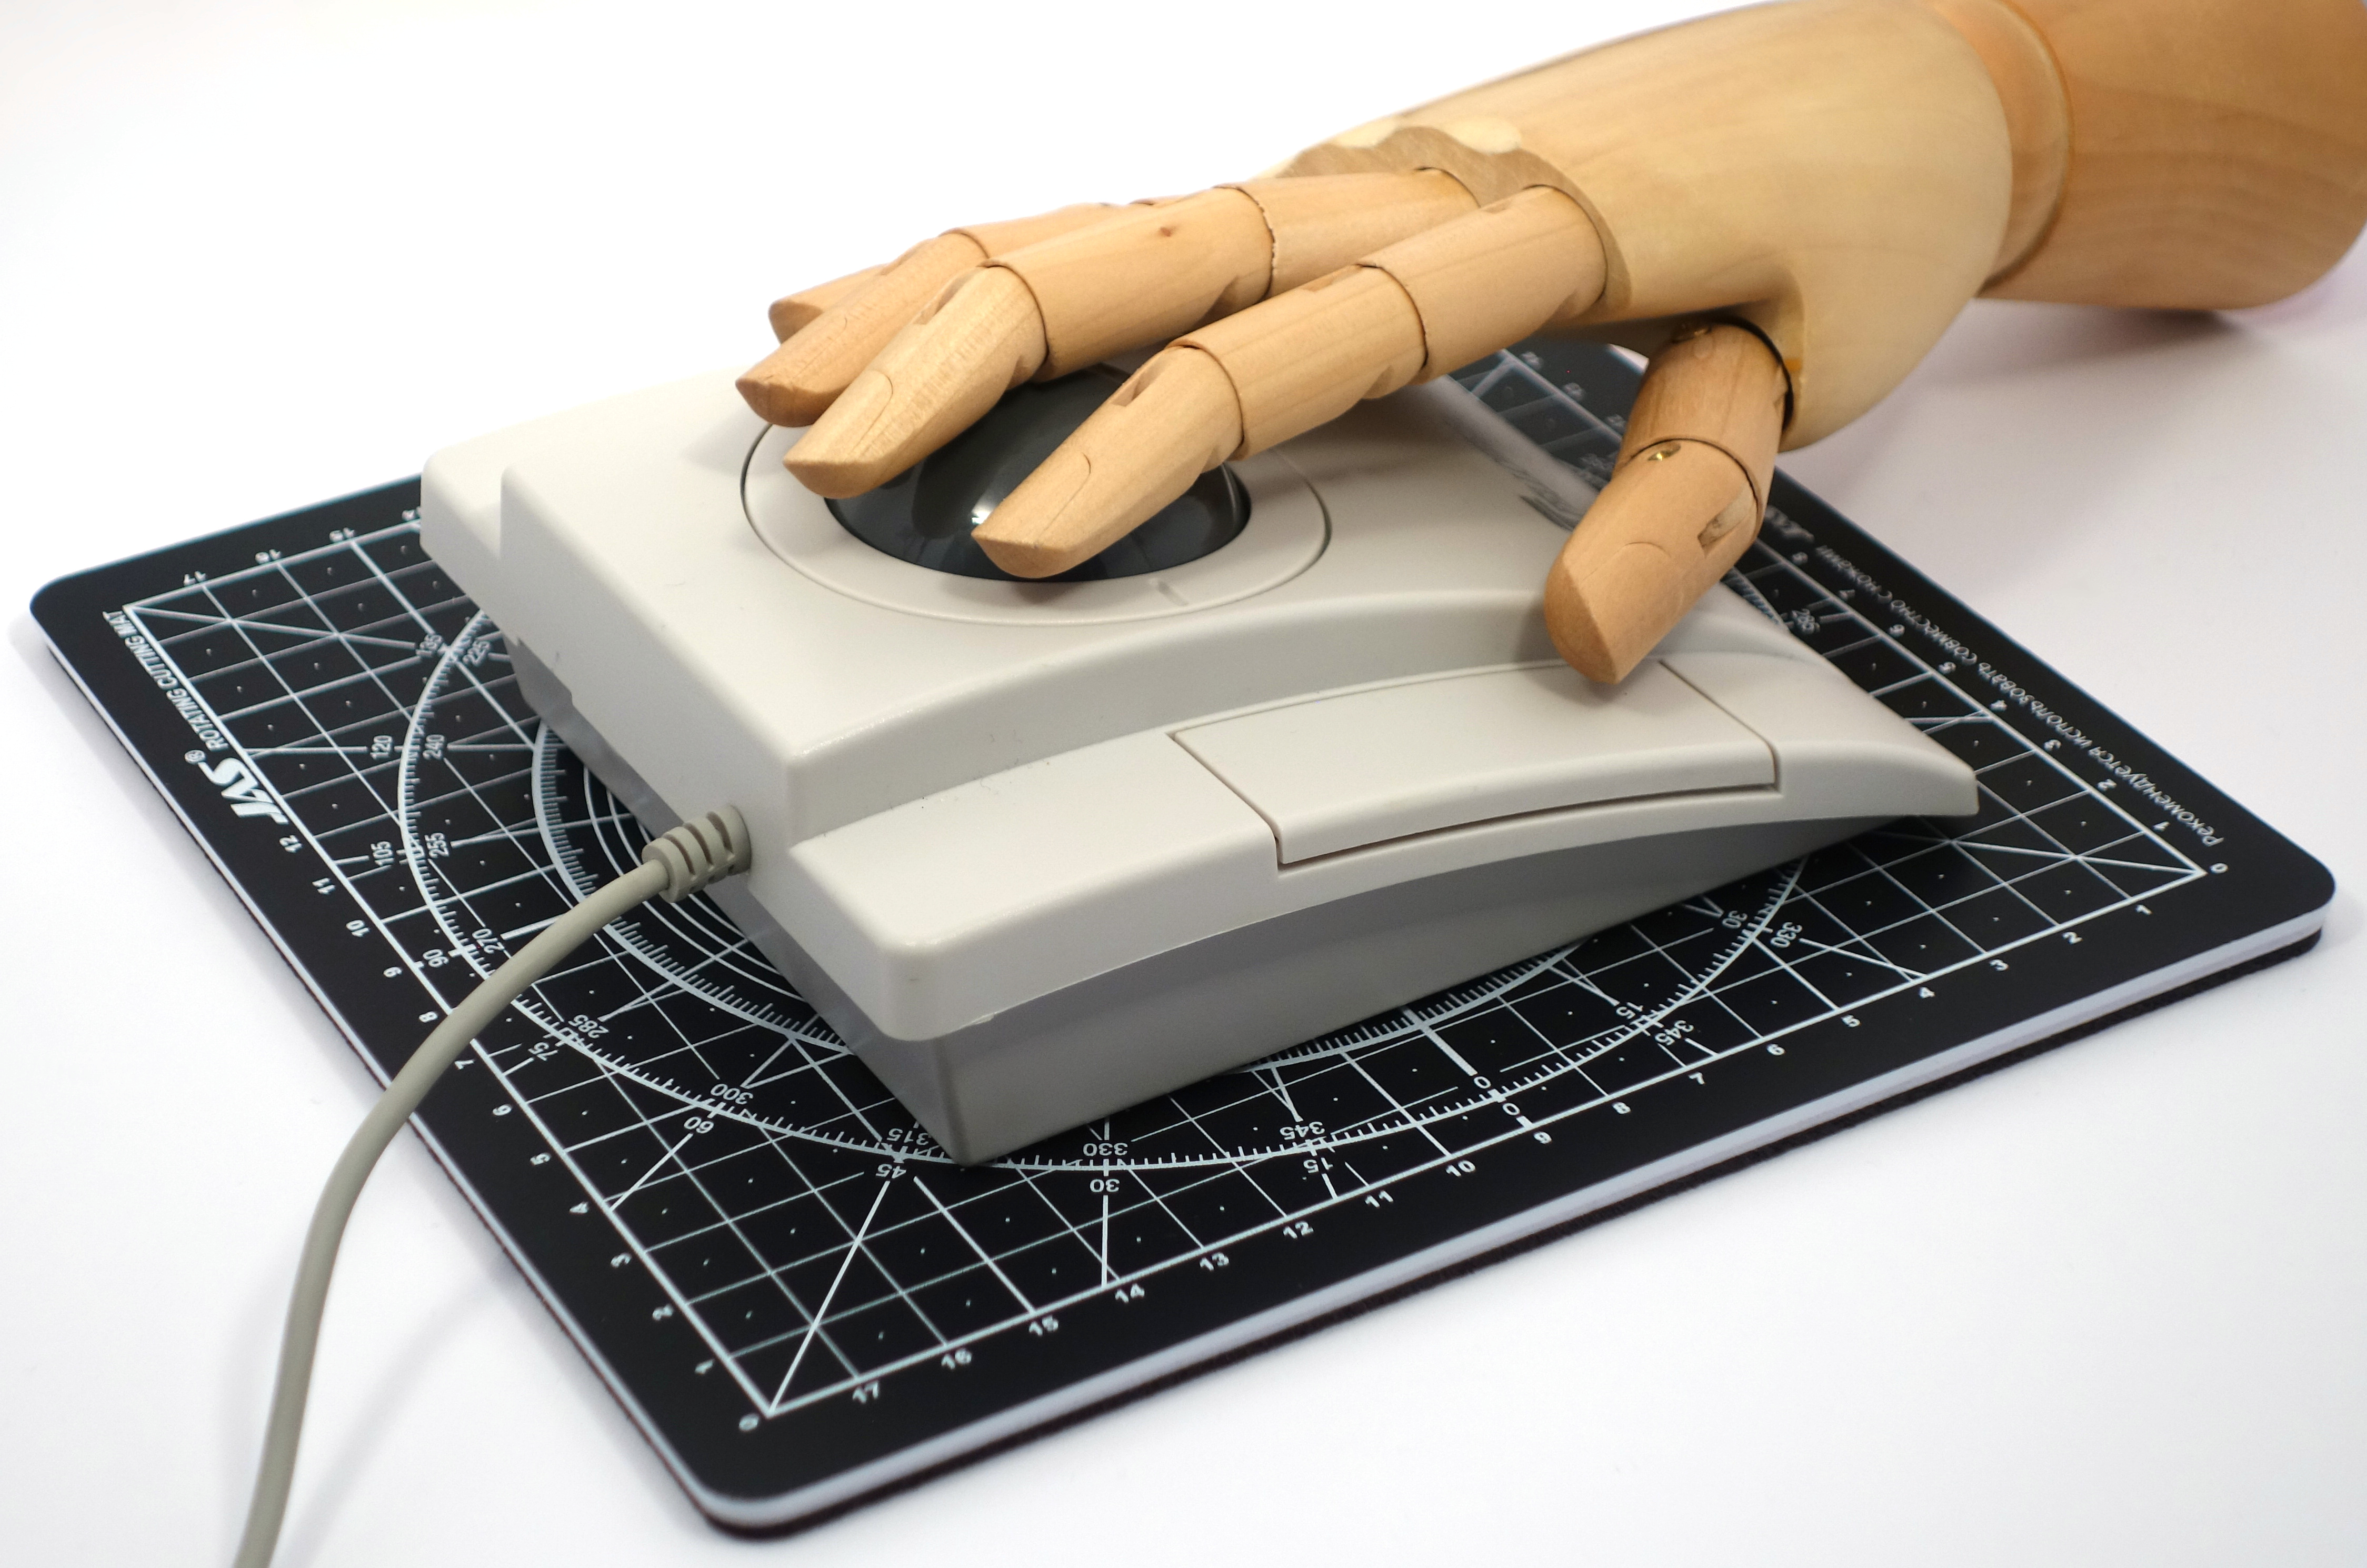
\includegraphics[scale=0.3]{1997_fellowes_trackball/hand_30.jpg}
    \caption{Fellowes Trackball с моделью руки человека}
    \label{fig:FellowesTrackballHand}
\end{figure}

В плане эргономики можно отметить удобную форму корпуса и кнопки большого размера, однако расположение кнопок нельзя назвать оптимальным (рис. \ref{fig:FellowesTrackballHand}). Использование всего двух кнопок, расположенных симметрично по бокам устройства, делает внешний вид эстетически привлекательным, однако это заставляет пользователя расставлять пальцы максимально широко ~--- особенно при необходимости их одновременного нажатия, которое, в теории, могло бы использоваться для имитации отсутствующей третьей кнопки либо для использования шара для скроллинга.

\begin{figure}[h]
    \centering
    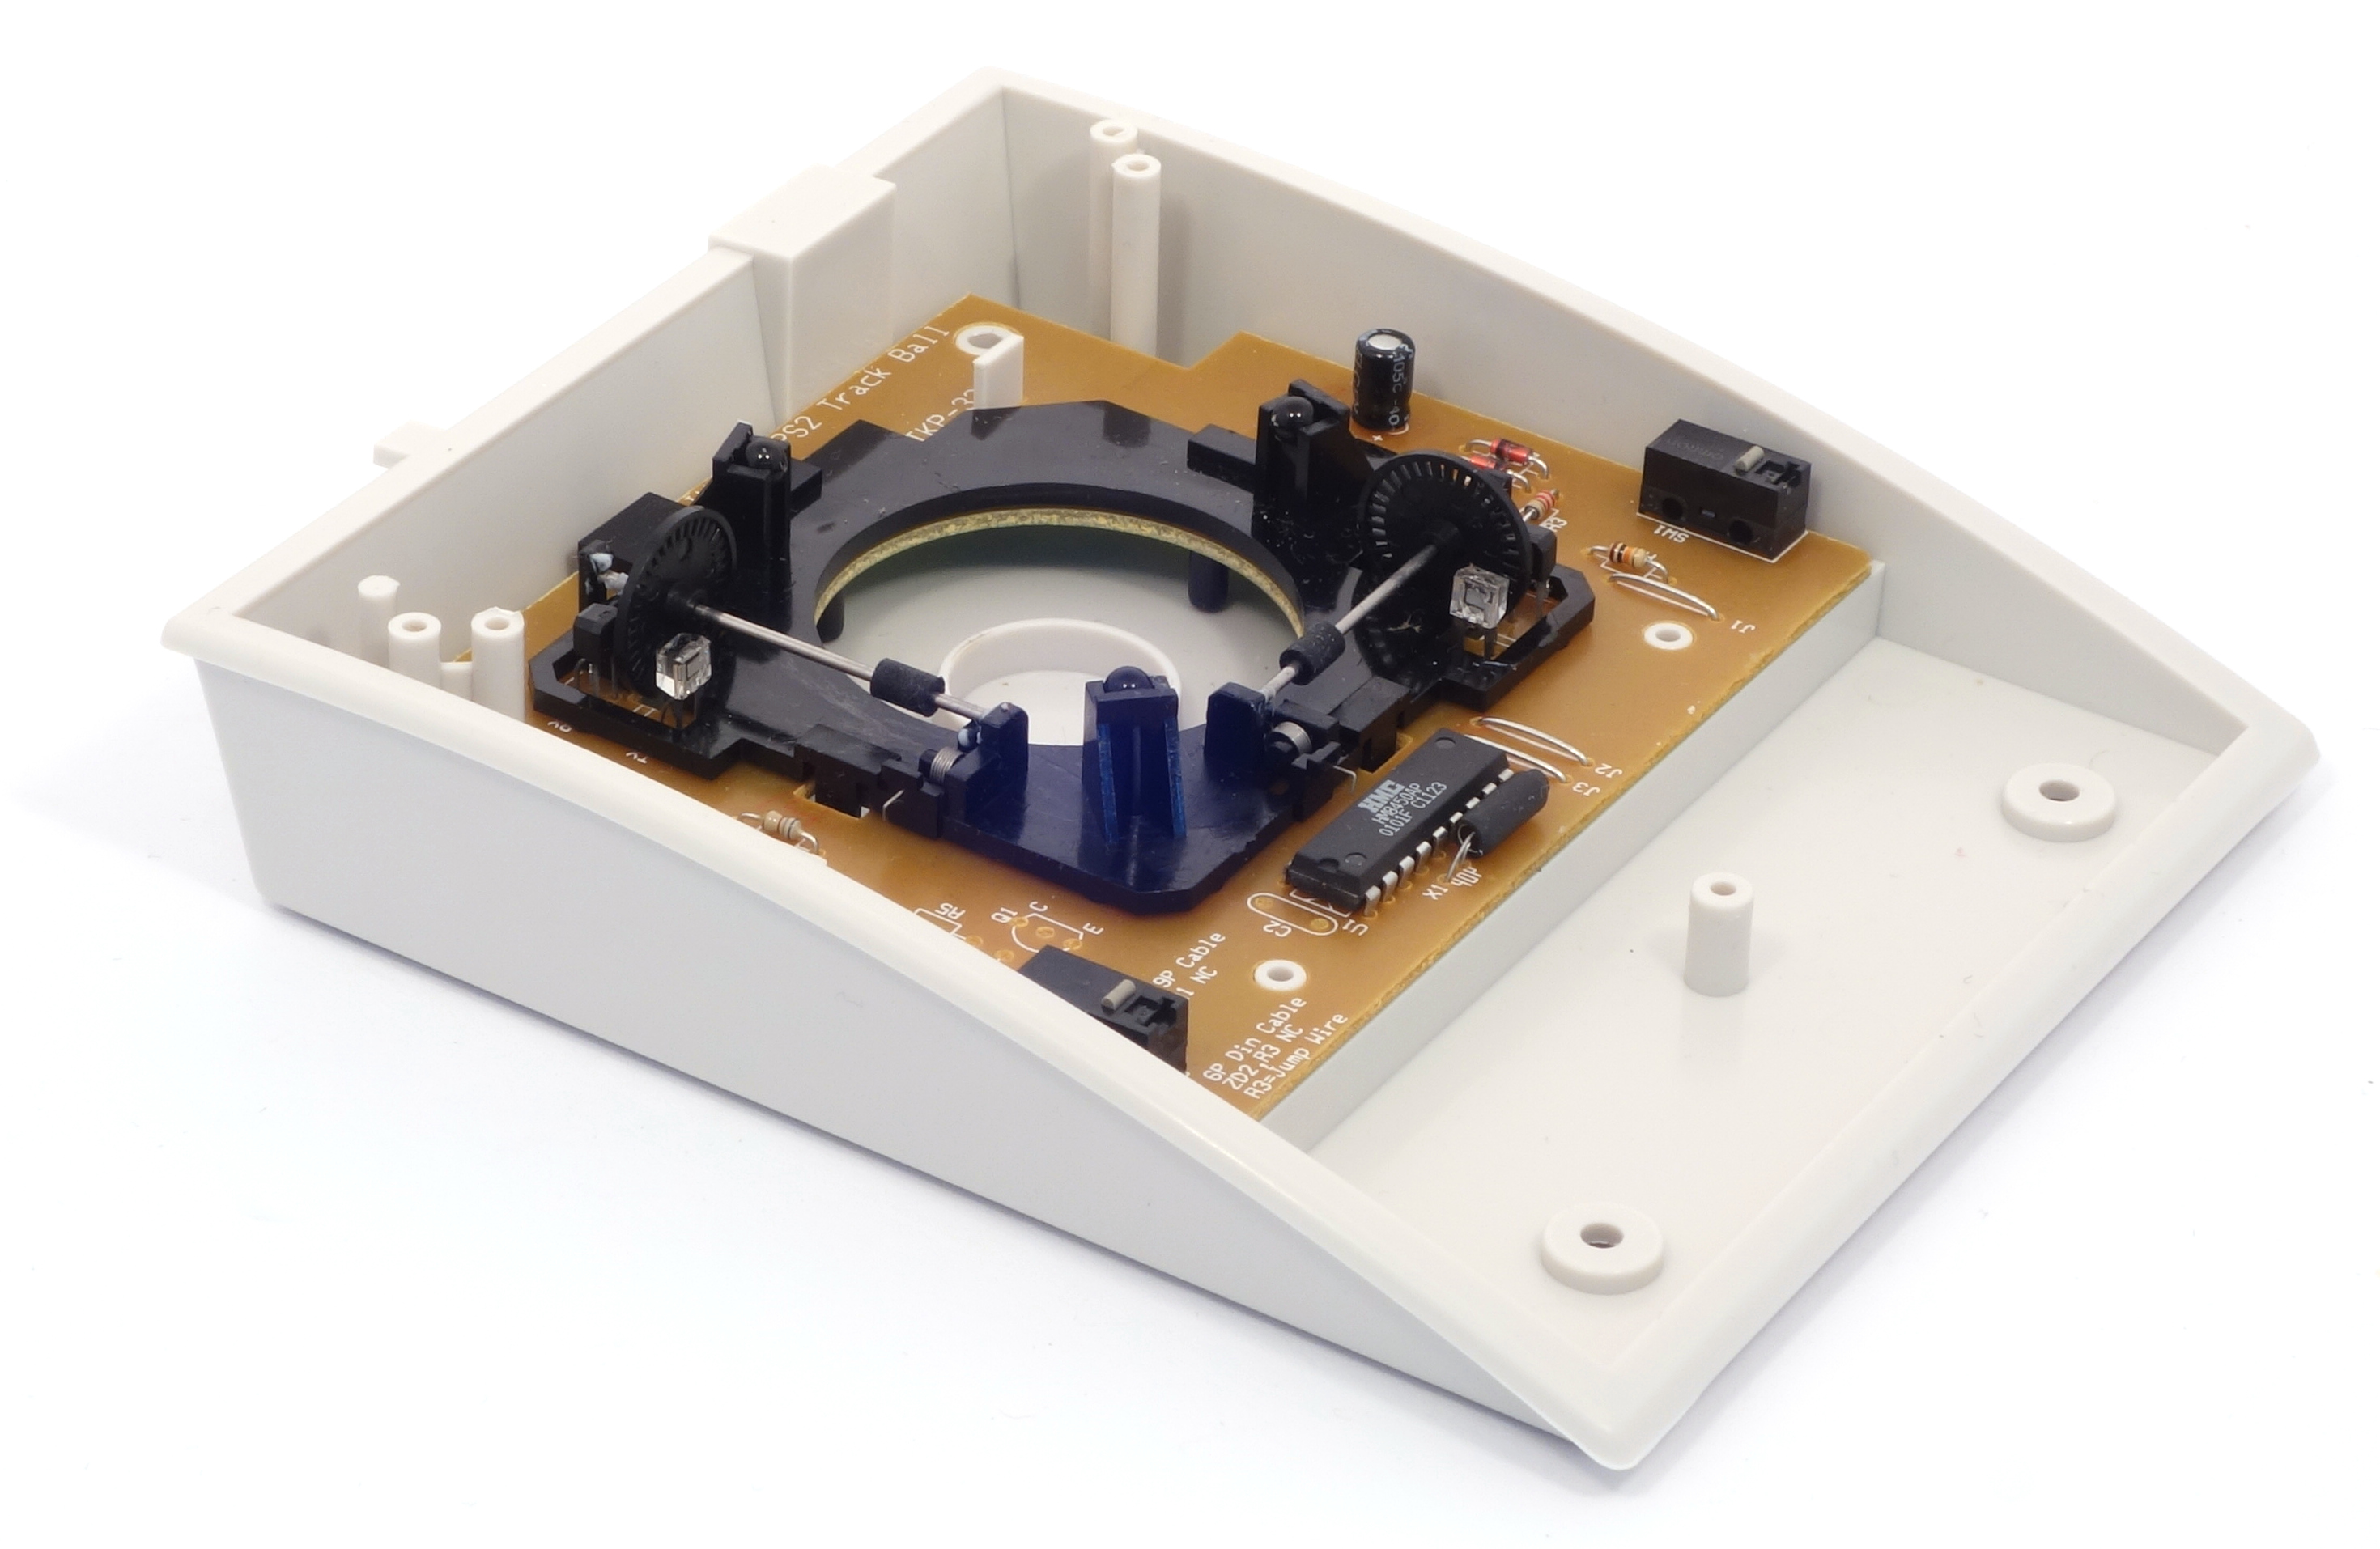
\includegraphics[scale=0.7]{1997_fellowes_trackball/inside_60.jpg}
    \caption{Fellowes Trackball в разобранном виде}
    \label{fig:FellowesTrackballInside}
\end{figure}

Внутреннее устройство данного трекбола показано на рис. \ref{fig:FellowesTrackballInside}. Как можно видеть,  трекбол выполнен по традиционной оптомеханической схеме. Помимо симметричного дизайна, одинаково удобного как для левой, так и для правой руки, производитель в рекламных материалах делал упор на высококачественные кнопки большой площади. В плане совместимости заявлена поддержка ОС Windows начиная с версии 3.1 \cite{advertising}.

\begin{thebibliography}{9}
\bibitem{advertising} Fellowes on-line catalog \url{https://docs.rs-online.com/046b/0900766b8024b417.pdf}
\end{thebibliography}
\end{document}
